\begin{figure}[t]
\centering
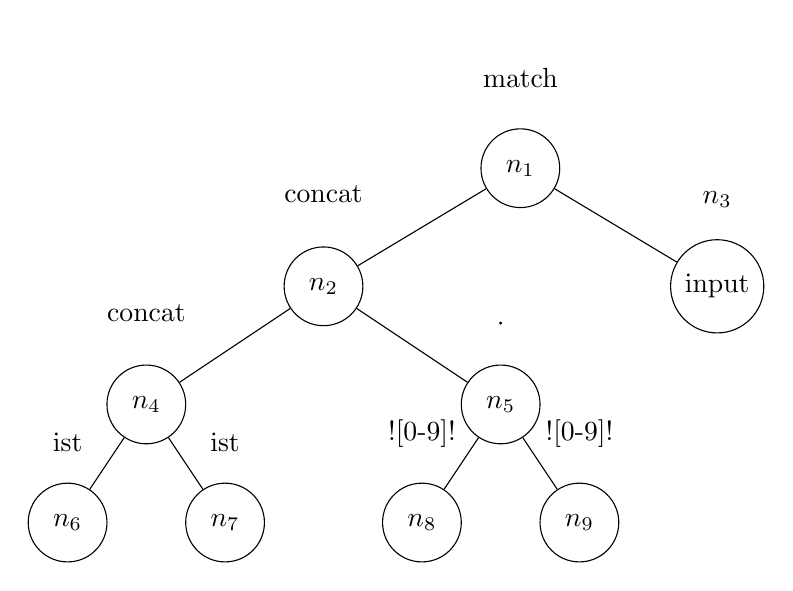
\begin{tikzpicture}[level distance=1.5cm,
level 1/.style={sibling distance=5cm},
level 2/.style={sibling distance=4.5cm},
level 3/.style={sibling distance=2cm}]
\tikzstyle{every node}=[circle,draw,minimum size=1cm]

\node (Root) [label={match}] {\(n_1\)}
child {
    node [label={concat}] {\(n_2\)} 
    child {
        node [label={concat}] {\(n_4\)}
        child { node [label={\regex{ist}}]{\(n_6\)} }
        child { node [label={\regex{ist}}]{\(n_7\)} } % edge from parent node[left, draw=none] {help!}
    }
    child {
        node [label={\(\boldsymbol{\cdot}\)}] {\(n_5\)}
        child { node [label={\Verb![0-9]!}] {\(n_8\)} }
        child { node [label={\Verb![0-9]!}] {\(n_9\)} }
    }
}
%
child {
    node [label={\(n_3\)}]{input}
};

\end{tikzpicture}
    \caption{Program tree for match validation with regular expression \regex{istist[0-9][0-9]}}
    \label{fig:example-regex-tree}
\end{figure}{}
